\selectlanguage{ngerman}%
\frenchspacing%
\begin{ledgroupsized}[r]{120mm}%
\footnotesize%
\pstart%
\noindent%
\textbf{Überlieferung:}%
\pend%
\end{ledgroupsized}%
\begin{ledgroupsized}[r]{114mm}%
\footnotesize%
\pstart%
\parindent -6mm%
\makebox[6mm][l]{\textit{L}}%
Aufzeichnung:
LH\;XXXV\;9,\;25 Bl.\;3.
Ein Blatt 4\textsuperscript{o};
Ränder teilweise beschnitten.
Zwei ganzseitig beschriebene Seiten.
\edlabel{LH_35_09_25_003_ubrlf-1}%
Die Aufzeichnung ist im Nachlass zwischen den Trägern des inhaltlich verwandten Entwurfs N.\;\ref{41212} (LH~XXXV~9,~25, Bl.\;1--2 und Bl.\;4--5) überliefert.%
\edlabel{LH_35_09_25_003_ubrlf-2}
\pend%
\end{ledgroupsized}%
\selectlanguage{latin}%
\frenchspacing%
\vspace{8mm}%
\normalsize%
\pstart%
\noindent%
\bracks{%
\href{\Scan{LH_35_09_25_003r}}%
{3\,r\textsuperscript{o}}%
}
\edlabel{LH_35_09_25_003_003r_nld-1}%
Die lufft in dem%
\indexS{Lufft, gepreßt}
\edtext{%
Cubischen Schuch \textit{AB}%
\indexS{Schuch, cubisch}%
}{%
\lemma{Cubischen Schuch \textit{AB}}%
\Cfootnote{%
Vgl. das Diagramm \lbrack\textit{Fig.\:1}\rbrack.
Der \textit{Schuh} als Maßeinheit der Länge entsprach im deutschsprachigen Raum dem \textit{Fuß}.%
}}
wird
\edtext{%
durch%
}{%
\lemma{durch}%
\Bfootnote{%
\textit{erg.\:L}%
}}
die last der obliegenden
\edtext{%
lufft,%
\indexS{Last der obliegenden Lufft}%
\indexS{Lufft, obliegend}
in dem stand%
}{%
\lemma{lufft,}%
\Bfootnote{%
\textit{(1)}~welche soviel th %
\textit{(2)}~in dem stand%
~\textit{L}%
}}
wie sich bey uns insgemein befindet%
\lbrack,\rbrack\
zusammen gehalten und gepreßet.
\edtext{%
Solche last beträgt%
\indexS{Last der obliegenden Lufft}%
}{%
\lemma{Solche}%
\Bfootnote{%
\textit{(1)}~last ist, %
\textit{(2)}~last beträgt%
~\textit{L}%
}}
soviel als 30 schuch waßer ohngefehr,%
\indexS{Waßer}
und
\edtext{%
ieder Cubischer schuch%
\indexS{Schuch, cubisch}%
}{%
\lemma{ieder}%
\Bfootnote{%
\textit{(1)}~schuch %
\textit{(2)}~Cubischer schuch%
~\textit{L}%
}}
waßer
gerechnet auff 70 Pfund,%
\indexS{Pfund}
\edtext{%
thut 2100 \Pfund.%
}{%
\lemma{thut}%
\Bfootnote{%
\textit{(1)}~3700 \Pfund\ %
\textit{(2)}~2100 \Pfund.%
~\textit{L}%
}}
Wolte man nun die lufft%
\indexS{Lufft, gepreßt}
in ein halb so enges Spatium preßen,
müste man dazu noch eins soviel gewicht haben,%
\indexS{Gewicht, von der Lufft getragen}
nehmlich 4200 \Pfund,
und hat also die in einen Cubischen schuch%
\indexS{Schuch, cubisch}
\edtext{%
\textit{AB} auß zwey in \textit{CB}%
}{%
\lemma{\textit{AB} auß zwey in \textit{CB}}%
\Bfootnote{%
\textit{erg.\;L}%
}}
gepreßete lufft soviel%
\indexS{Lufft, gepreßt}
\edtext{%
krafft,%
\indexS{Krafft der gepreßten Lufft}
daß sie das gewicht von 4200 \Pfund\ in vacuo%
\indexS{vacuum}%
\indexS{in vacuo}
tragen kan,%
}{%
\lemma{krafft,}%
\Bfootnote{%
\textit{(1)}~als 4200 \Pfund, so %
\textit{(a)}~aus %
\textit{(b)}~von \textit{C} bis \textit{A}
\bars{herab \textit{streicht Hrsg.}} fallen, und %
\textit{(2)}~daß sie %
\bars{das gewicht von \textit{erg.}} 4200 \Pfund\ %
\bars{in vacuo \textit{erg.}} tragen kan,%
~\textit{L}%
}}
und gesezt
man konne 10 mahl soviel lufft hinein preßen,%
\indexS{Lufft, gepreßt}
so
\edtext{%
kondte solche lufft hernach 21000 \Pfund\ tragen.%
\indexS{Gewicht, von der Lufft getragen}%
\edlabel{LH_35_09_25_003_003r_nld-2}%
}{%
\lemma{kondte}%
\Bfootnote{%
\textit{(1)}~sie 21000 \Pfund\ %
\textit{(2)}~solche lufft hernach 21000 \Pfund\ tragen.%
~\textit{L}%
}}
Weilen aber die krafft der sich wieder stellenden lufft%
\indexS{Krafft der sich wieder stellenden Lufft}
zu meßen
nicht gnug ist,
daß man wiße
wieviel sie tragen %
oder noch wohl in die höhe heben könne,
sondern auch wie hoch;
so ist
\edtext{%
zu bedencken,%
}{%
\lemma{zu}%
\Bfootnote{%
\textit{(1)}~wißen, %
\textit{(2)}~bedencken%
~\textit{L}%
}}
daß wenn man
\edtext{%
in vacuo%
\indexS{vacuum}%
\indexS{in vacuo}%
}{%
\lemma{in vacuo}%
\Bfootnote{\textit{erg.\;L}%
}}
anstatt der
\edtext{%
4200 \Pfund,
so%
}{%
\lemma{4200 \Pfund,}%
\Bfootnote{%
\textit{(1)}~nur %
\textit{(2)}~so%
~\textit{L}%
}}
die lufft \textit{CB} in \textit{AB} halten,
nur 2100 darauff legte
\edtext{%
in \textit{D},%
}{%
\lemma{in \textit{D}}%
\Bfootnote{\textit{erg.\;L}%
}}
sich die lufft restituiren werde%
\indexS{Lufft, sich restituirend}
aus \textit{AB} in \textit{CB},
und das gewicht bis dahin heben,%
\indexS{Gewicht, von der Lufft getragen}
welches
\edtext{%
dann durch den erlangten Schwung%
\indexS{Schwung, erlangt}
noch sich selbst werde steigen können.%
}{%
\lemma{dann}%
\Bfootnote{%
\textit{(1)}~auch eine mehrere krafft %
\textit{(2)}~durch den erlangten Schwung %
\textit{(a)}~hernach %
\textit{(b)}~vor dann %
\textit{(c)}~noch sich %
\lbrack...\rbrack\ steigen können.%
~\textit{L}%
}}
Wie hoch aber,
das wäre
\edtext{%
auszurechnen,
und daher ein gewicht%
\indexS{Gewicht, von der Lufft getragen}
zu finden,
welches
durch einen fall%
\indexS{Fall}
aus einer gewissen Hohe%
\indexS{Hohe des Falles}
praecise die lufft%
\indexS{Lufft, gepreßt}
aus \lbrack\textit{CB}\rbrack\
in \lbrack\textit{AB}\rbrack\
preßen köndte.
Nun ist das gewicht \textit{D} von 2100 \Pfund%
\indexS{Pfund}%
}{%
\lemma{auszurechnen}%
\Bfootnote{%
\textit{(1)}~. Es ist nehmlic %
\textit{(2)}~. Es ist aber das das\lbrack\textit{!}\rbrack\ pondus \textit{D} von 2100 pfunden %
\textit{(3)}~. Solches wäre aus %
\textit{(4)}~, und daher %
\lbrack...\rbrack\ die lufft %
\textit{(a)}~bis %
\textit{(b)}~aus %
\bars{\textit{CD} \textit{ändert Hrsg.}} in %
\bars{\textit{AD} \textit{ändert Hrsg.}} preßen köndte. Nun %
\textit{(aa)}~das %
\textit{(bb)}~ist das %
\lbrack...\rbrack\ 2100 \Pfund%
~\textit{L}%
}}
und fallet aus \textit{C} bis \textit{A},
so kan es solches nicht verrichten;
ist es aber von 4200 \Pfund,
und fället von \textit{C} bis \textit{A},
so kan es ein weit mehrers Verrichten,
und wurde
in \textit{A} nicht bleiben.
Ja es falle das
\edtext{%
gewicht%
\indexS{Gewicht, von der Lufft getragen}
\lbrack4200\rbrack\
von was für kleiner hohe \textit{EA}%
\indexS{Hohe des Falles}%
}{%
\lemma{gewicht}%
\Bfootnote{%
\textit{(1)}~\textit{E} von was fur klei %
\textit{(2)}~\textit{D} vo %
\textit{(3)}~von %
\textit{(4)}~\bars{42100 \textit{ändert Hrsg.}} von was %
\lbrack...\rbrack\ hohe \textit{EA}%
~\textit{L}%
}}
es wolle,
wird es doch durch den schwung%
\indexS{Schwung, erlangt}
etwas unter \textit{A} herabsteigen,
wiewohl es hernach wieder wird hinauff müßen.
\pend%
\begin{edfigure}[2.75em][2.0em]%
\hspace*{-50mm}%
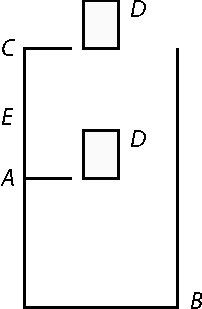
\includegraphics[width=0.22\textwidth]
{gesamttex/edit_VIII-4/images/LH_35_09_25_003_d1_003r.pdf}
\edcaption[0.25em]{%
\hspace*{-50mm}%
\lbrack\textit{Fig.\:1}\rbrack%
}%
\vspace{-13.00em}%
\hspace*{50mm}%
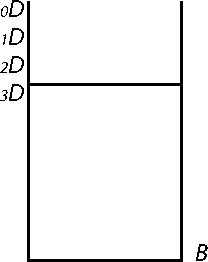
\includegraphics[width=0.23\textwidth]
{gesamttex/edit_VIII-4/images/LH_35_09_25_003_d2_003r.pdf}
\edcaption[0.25em]{%
\hspace*{50mm}%
\lbrack\textit{Fig.\:2}\rbrack%
}%
\end{edfigure}%
\pstart%
Demnach muß
\edtext{%
man die hohe des falles%
\indexS{Hohe des Falles}
unendtlich klein nehmen,%
}{%
\lemma{man}%
\Bfootnote{%
\textit{(1)}~\textit{EA} unendtlich klein nehmen %
\textit{(2)}~die hohe %
\lbrack...\rbrack\ klein nehmen,%
~\textit{L}}}
und sezen,
daß das fallende corpus%
\indexS{corpus, fallend}
\edtext{%
immer
weren\lbrack d \rbrack dem
fallen%
}{%
\lemma{immer}%
\Bfootnote{%
\textit{(1)}~we %
\textit{(2)}~wehr %
\textit{(3)}~\bars{werendem \textit{ändert Hrsg.}} fallen%
~\textit{L}%
}}
wachse,
\edtext{%
wurde der calculus%
\indexS{calculus, angestellet}
also%
}{%
\lemma{wurde}%
\Bfootnote{%
\textit{(1)}~\bars{also \textit{streicht Hrsg.}} %
\textit{(2)}~der calculus also%
~\textit{L}%
}}
angestellet werden konnen.
Das gewicht \textit{\ind{1}D}%
\indexS{Gewicht, von der Lufft getragen}
ist der lufft feder gleich%
\indexS{Lufft}%
\indexS{Feder der Lufft}
und drückt sie
\edtext{%
derowegen hinab%
}{%
\lemma{derowegen}%
\Bfootnote{%
\bars{von \textit{\ind{1}D} \textit{gestr.}} hinab%
~\textit{L}%
}}
in \textit{\ind{2}D},
also daß
\textit{\ind{1}D}\textit{\ind{2}D}
unendtlich%
\indexS{Fall, unendtlich klein}
\edtext{%
klein sey.
\textit{B}\textit{\ind{1}D}
sey \textit{x},
so ware die lufft feder%
\indexS{Lufft}%
\indexS{Feder der Lufft}
$\dfrac{1}{x}$,%
}{%
\lemma{klein sey.}%
\Bfootnote{%
\textit{(1)}~\bars{Wir sollen \textit{streicht Hrsg.}} %
\textit{(2)}~Sey der lufft feder\indexS{Feder der Lufft}\indexS{Lufft} %
\textit{(3)}~\textit{B}\textit{\ind{1}D} sey %
\lbrack...\rbrack\ feder $\dfrac{1}{x}$,%
~\textit{L}%
}}
ferner das Spatium
\textit{\ind{1}D}\textit{\ind{2}D}
ist $d\overline{x}$,
so
\edtext{%
ware die lini \textit{B}\textit{\ind{2}D}
soviel als $x - d\overline{x}$
und die lufft feder%
\indexS{Lufft}%
\indexS{Feder der Lufft}%
}{%
\lemma{ware die}%
\Bfootnote{%
\textit{(1)}~lufft feder %
\textit{(2)}~lini \textit{B}\textit{\ind{2}D} %
\lbrack...\rbrack\ lufft feder%
~\textit{L}%
}}
in \textit{B}\textit{\ind{2}D}
soviel als $\dfrac{1}{x - d\overline{x}}$,%
\ledpb
und müßen wir derowegen das gewicht \textit{\ind{1}D}%
\indexS{Gewicht, von der Lufft getragen}%
\indexS{Gewicht, vermehrt}
soviel vermehren in~\textit{\ind{2}D},
daß es solcher lufft feder gleich%
\indexS{Lufft}%
\indexS{Feder der Lufft}
und also sey $\dfrac{1}{x-d\overline{x}}$,
auff welchen fall es fallen konne
\edtext{%
bis \textit{\ind{3}D},
das augmentum ponderis%
\indexS{augmentum ponderis}
aber ware
$\dfrac{d\overline{x}}{xx}$.
\bracks{%
\href{\Scan{LH_35_09_25_003v}}%
{3\,v\textsuperscript{o}}%
}
\edtext{}{%
\lemma{\textit{Am oberen Blattrand, gestrichen:}}%
\Afootnote{%
Das beste wäre sezen
daß man das pondus allzeit lasse.%
\indexS{pondus, fallend}%
}}%
Wenn nun das pondus $\dfrac{\pi}{x}$%
\indexS{pondus, fallend}
fallend von der Höhe \textit{\ind{1}D},%
\indexS{Hohe des Falles}
capabel ist die lufft%
\indexS{Lufft, gepreßt}
deren vis Elastica%
\indexS{vis elastica der Lufft}
$\dfrac{\varepsilon}{x}$,
so zu preßen von \textit{\ind{1}D}
bis \textit{\ind{2}D}
durch das Spatium $d\overline{x}$,%
so wird das pondus $\dfrac{\pi}{x + d\overline{x}}$,
fallende von der hohe \textit{\ind{2}D},%
\indexS{pondus, fallend}
capabel seyn
die lufft%
\indexS{Lufft, gepreßt}
deren vis Elastica%
\indexS{vis elastica der Lufft}
$\displaystyle\dfrac{\varepsilon}{x + d\overline{x}}$
zu preßen durch das Spatium $(d\overline{x})$
oder \textit{\ind{2}D}\textit{\ind{3}D},
und $(d\overline{x})$ wird seyn zu $d\overline{x}$
in ratione composita
\rule[0mm]{0mm}{4.0mm}%
ex directa ponderum
et reciproca virium Elasticarum%
\indexS{vis elastica aeris}
seu
$\displaystyle\dfrac{(d\overline{x})}{d\overline{x}}=\dfrac{\pi}{x}$ ad $\displaystyle\dfrac{\pi}{x + d\overline{x}}$ in $\dfrac{\varepsilon}{x + d\overline{x}}$ ad $\displaystyle\dfrac{\varepsilon}{x}$,
seu
$\displaystyle\dfrac{(d\overline{x})}{d\overline{x}}=1$.
\rule[0mm]{0mm}{5.4mm}%
Ergo aucto pondere,%
\indexS{pondus comprimens aerem}%
\indexS{pondus auctum}
ut sit semper vi Elasticae%
\indexS{vis elastica aeris}
aequale%
\lbrack,\rbrack\
erunt incrementa spatiorum aequalia.%
\indexS{incrementum spatii}%
}{%
\lemma{bis \textit{\ind{3}D},}%
\Bfootnote{%
\textit{(1)}~we %
\textit{(2)}~und weil wir konnen sezen %
\textit{(a)}~\textit{x} %
\textit{(b)}~$\ind{1}D\ind{2}D = \ind{2}D\ind{3}D$, so muste das pondus in \textit{\ind{3}D} wieder vermehrt werden, daß es stiege auff $\dfrac{1}{x-3d\overline{x}}$ und so fort, bis man aufhohren will %
\textit{(3)}~das augmentum %
\lbrack...\rbrack\ ware $\dfrac{d\overline{x}}{xx}$. %
\textit{(a)}~Wenn nun das pondus $\dfrac{1}{x}$ fallend von der hohe \textit{\ind{0}D}\textit{\ind{1}D} %
\textit{(aa)}~hat %
\textit{(bb)}~macht die lufft feder \textit{B}\textit{\ind{1}D} ein zu preßen bis \textit{\ind{2}D} \href{\Scan{LH_35_09_25_003v}}{\lbrack3\,v\textsuperscript{o}\rbrack} quaeritur wie weit %
\textit{(b)}~Wenn nun das pondus %
\textit{(aa)}~$\dfrac{\pi}{x}$ fallende %
\textit{(bb)}~$\dfrac{\pi}{x}$ fallend %
\lbrack...\rbrack\ die lufft %
\textit{(aaa)}~deren vis Elastica $\dfrac{\pi}{x}$, %
\textit{(bbb)}~deren vis Elastica $\dfrac{\pi}{x}$, %
\textit{(ccc)}~deren vis Elastica $\dfrac{\varepsilon}{x}$, so %
\textit{(aaaa)}~weit zu preßen bis in \textit{\ind{2}D} %
\textit{(bbbb)}~zu preßen von \textit{\ind{1}D} bis \textit{\ind{2}D} %
\textit{(aaaaa)}~und %
\textit{(bbbbb)}~q %
\textit{(ccccc)}~durch das %
\lbrack...\rbrack\ so wird %
\textit{(aaaaa-a)}~die lufft %
\textit{(bbbbb-b)}~das pondus %
\lbrack...\rbrack\ durch das Spatium %
\textit{(aaaaa-aa)}~$(d\overline{x})$, welches %
\textit{(bbbbb-bb)}~$(d\overline{x})$ oder \textit{\ind{2}D}\textit{\ind{3}D},%
\textit{(aaaaa-aaa)}~welches %
\textit{(bbbbb-bbb)}~und dergestalt weil %
\textit{(ccccc-ccc)}~und $(d\overline{x})$ wird %
\lbrack...\rbrack\ ponderum et reciproca %
\textit{(aaaaa-aaaa)}~distantiarum %
\textit{(bbbbb-bbbb)}~virium Elasticarum %
\lbrack...\rbrack\ seu $\displaystyle\dfrac{(d\overline{x})}{d\overline{x}}=1$. Ergo %
\textit{(aaaaa-aaaaa)}~auctore %
\textit{(bbbbb-bbbbb)}~aucto pondere, %
\lbrack...\rbrack\ spatiorum aequalia.%
~\textit{L}%
}}
\rule[0mm]{0mm}{3.9mm}%
Jam
\edtext{%
vi\lbrack re\rbrack s%
}{%
\lemma{vis}%
\Bfootnote{%
\textit{L\;ändert Hrsg.}%
}}
Elasticae sunt%
\indexS{vis elastica aeris}
$\dfrac{\varepsilon}{x}$
quarum differentiae $\dfrac{\varepsilon}{xx}$,
\rule[0mm]{0mm}{5.4mm}%
erunt ergo incrementa%
\indexS{incrementum ponderis}
\edtext{%
ponderum reciproce
ut quadrata spatiorum recipientium,%
}{%
\lemma{ponderum}%
\Bfootnote{%
\textit{(1)}~ut quadrata spatiorum 
\textit{(a)}~contrahentium, %
\textit{(b)}~recipientium, %
\textit{(2)}~reciproce ut quadrata spatiorum recipientium,%
~\textit{L}%
}}
\rule[0mm]{0mm}{3,4mm}%
aggregata autem%
\indexS{aggregatum}
seu pondera acquisita%
\indexS{pondus acquisitum}
erunt reciproce
\rule[0mm]{0mm}{5.2mm}%
ut spatia.
\pend%
\newpage%
\vspace*{0.75em}%
\begin{edfigure}[0.0em][1.75em]%
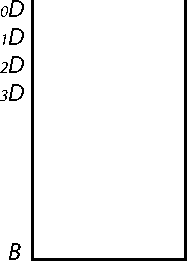
\includegraphics[width=0.21\textwidth]
{gesamttex/edit_VIII-4/images/LH_35_09_25_003_d3_003v.pdf}
\edcaption[0.25em]{%
\hspace*{4mm}%
\lbrack\textit{Fig.\:3}\rbrack%
}%
\end{edfigure}%
\pstart%
Sit ergo
\edtext{%
Hyperbola%
\indexS{hyperbola}%
}{%
\lemma{Hyperbola}%
\Cfootnote{%
Vgl. das Diagramm \lbrack\textit{Fig.\:4}\rbrack.%
}}
\edtext{%
cujus asymptotis \textit{BX},%
\indexS{asymptotos}
ordinatae%
}{%
\lemma{cujus}%
\Bfootnote{%
\textit{(1)}~ordinata %
\textit{(2)}~asymptotis \textit{BX}, ordinatae%
~\textit{L}%
}}
ad asymptoton $X\varPi$,
et
\edtext{%
sit in vacuo vas \textit{BC}%
\indexS{vas in vacuo}%
\indexS{vas comprimendum}%
\indexS{vacuum}%
}{%
\lemma{sit}%
\Bfootnote{%
\textit{(1)}~vas %
\textit{(2)}~in vacuo vas 
\textit{(a)}~\textit{AB} %
\textit{(b)}~\textit{BC}%
~\textit{L}%
}}
comprimendum a pondere%
\indexS{pondus comprimens vas}
$\varPi X$
continue augendo,%
\indexS{pondus augendum}
quantum opus est
\edtext{%
ut tum ab impetu concepto,%
\indexS{impetus conceptus}
tum a pondere accedente%
\indexS{pondus accedens}
continuetur%
}{%
\lemma{ut}%
\Bfootnote{%
\textit{(1)}~continuetur %
\textit{(2)}~tum ab %
\lbrack...\rbrack\ accedente continuetur%
~\textit{ L}}}
compressio%
\indexS{compressio aeris in vase}
usque
\edtext{%
ad \textit{A}.
Erunt gravitates%
\indexS{gravitas comprimens}%
}{%
\lemma{ad \textit{A}.}%
\Bfootnote{%
\textit{(1)}~Hinc erit %
\textit{(2)}~Erunt %
\textit{(a)}~continue %
\textit{(b)}~gravitates%
~\textit{L}%
}}
seu pondera%
\indexS{pondus comprimens vas}
ubique
ut ipsae $X\varPi$ ordinatae Hyperbolae,%
\indexS{hyperbola}
si ponamus primum pondus fuisse praecise
quale oportet
ut%
\lbrack,\rbrack\
si non augeretur%
\lbrack,\rbrack\
non amplius
comprimeret in\;\textit{C},
sed sustineretur.%
\indexS{pondus sustentum ab aere}
Quaeritur jam
quodnam pondus aequabile seu constans,%
\indexS{pondus aequabile}%
\indexS{pondus constans}
ex eadem altitudine \textit{CA} cadens%
\indexS{pondus cadens}%
\indexS{altitudo casus}
eundem effectum praestare potuisset.%
\indexS{effectus praestitus}
Aestimandum erit centrum gravitatis descensus%
\indexS{centrum gravitatis descensus}
seu summa descensus aequivalentis.%
\indexS{summa descensus aequivalentis}%
\indexS{descensus aequivalens}
Ponamus
\edtext{%
$CX = [X\varPi]$, 
dico pondus constans%
\indexS{pondus constans}%
}{%
\lemma{$CX\ =$}\Bfootnote{%
\bars{\textit{XP} \textit{ändert Hrsg.}} dico
\bars{dico \textit{gestr.}} pondus %
\textit{(1)}~uniforme\indexS{pondus uniforme} %
\textit{(2)}~constans%
~\textit{L}%
}}
quod ex \textit{C} cadens in \textit{A}%
\indexS{pondus cadens}
comprimit aerem \textit{CB}%
\indexS{pondus comprimens aerem}
in \textit{AB}
nec ultra esse ad pondus aliud constans%
\indexS{pondus constans}
quod ex \textit{C} cadens in \textit{((A))}%
\indexS{pondus cadens}
comprimit aerem \textit{CB}%
\indexS{pondus comprimens aerem}
in \textit{((A))B}
fore
\edtext{%
ut quadrilineum $\varPi CA\textit{(X)}$%
\indexS{quadrilineum}
divisum per \textit{CA}
ad quadrilin. $\varPi C\textit{((A))((X))}$%
\indexS{quadrilineum}
divisum per \textit{C((A))}.
Nimirum vis%
\indexS{vis effecta a corpore descendente}
quam efficit corpus
dicto modo auctum%
\indexS{corpus auctum}
suo descensu%
\indexS{descensus corporis comprimentis}
est
tum $X\varPi$ prima
seu \textit{CX} ductum in \textit{CA},%
}{%
\lemma{ut}%
\Bfootnote{%
\textit{(1)}~quinquilineum\indexS{quinquilineum} %
\textit{(2)}~quadrilineum $\varPi CA\textit{(X)}$ %
\bars{%
\textit{(1)}~ductum in %
\textit{(2)}~divisum per \textit{CA} %
\textit{erg.}} ad quadrilin. %
\lbrack...\rbrack\ \textit{C((A))}. Nimirum %
\textit{(a)}~corpus $X\varPi$ %
\textit{(b)}~vis quaesita descen\indexS{vis quaesita descensu} %
\textit{(c)}~vis quam %
\lbrack...\rbrack\ est tum
\textit{(aa)}~\textit{X} du %
\textit{(bb)}~$X\varPi$ 
\textit{(aa)}~ductum %
\textit{(bb)}~prima %
\textit{(aaa)}~du %
\textit{(bbb)}~seu \textit{CX} ductum in \textit{CA},%
~\textit{L}%
}}
tum differentia quaelibet
quae est
$\dfrac{\varPi}{xx} d\overline{x}$
ducta in \textit{x},
quae facit
$\dfrac{\varPi}{x}d\overline{x}$.
\pend%
\newpage%
\begin{edfigure}[0.0em][1.0em]%
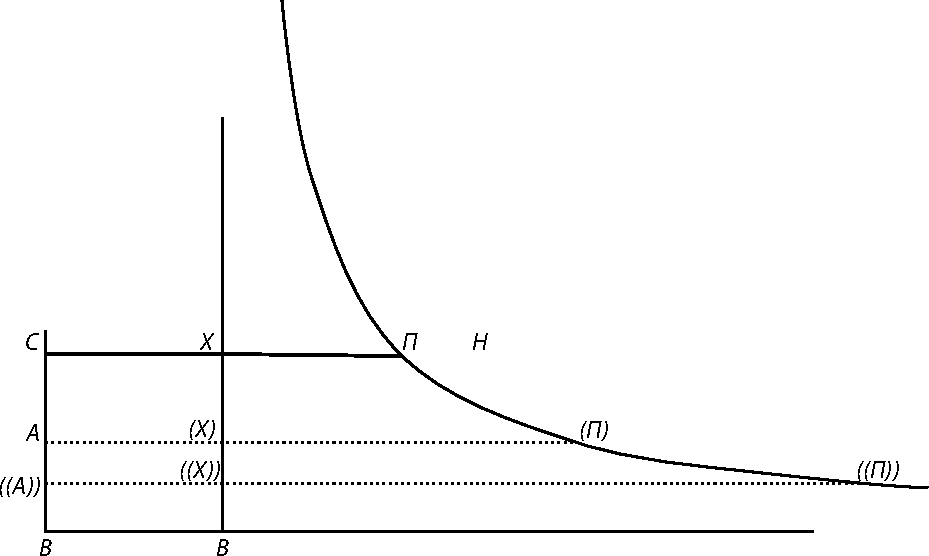
\includegraphics[width=0.94\textwidth]
{gesamttex/edit_VIII-4/images/LH_35_09_25_003-d4_003v.pdf}
\edcaption[0.25em]{%
\lbrack\textit{Fig.\:4}\rbrack%
\edtext{}{%
\lemma{\textit{Zum Diagramm} \lbrack\textit{Fig.\:4}\rbrack:}%
\Afootnote%
[nonum]%
{%
$BX = 1 = [X\varPi]\textsuperscript{[\text{a}]} = XC$.
\quad%
$B\textit{(X)} = \dfrac{1}{10}$.
\quad%
$\varPi \textit{X(X)}\varPi$
circiter est $18 + \dfrac{1}{\langle25\rangle}$,
dividatur per \textit{CA} 
seu $\dfrac{10}{9}$
fit circiter $\dfrac{167}{100}$,%
\textsuperscript{[b]}
cui addatur
\textit{CX} seu 1,
fit $\dfrac{267}{100}$,
multiplicanda per 2100
fit 267 per 21,
pondus quod cadens ex alt. \textit{CA}%
\indexS{altitudo casus}
$\dfrac{10}{9}$ pedis in vacuo%
\indexS{pes}%
\indexS{vacuum}%
\indexS{in vacuo}
deprimere potest aerem.%
\indexS{pondus deprimens aerem}
\\[1.5ex]%
{\footnotesize%
\textsuperscript{[a]}~\textit{XP} \textit{L ändert Hrsg.}
\quad%
\textsuperscript{[b]}~circiter $\dfrac{167}{100}$:
Das ungefähre Ergebnis ist um den Faktor 10 zu klein.%
}%
}}%
}%
\pagelabel{LH_35_09_25_003_003v_Fig4}%
\end{edfigure}
\pstart%
\noindent%
\edlabel{LH_35_09_25_003_003v_nld-1}%
Ergo summa differentiarum
in suos descensus ductarum%
\indexS{descensus corporis comprimentis}
est
$\displaystyle\varPi\!\!\int\!\!\dfrac{1}{x}$
\edtext{%
seu repraesentatur%
}{%
\lemma{seu}%
\Bfootnote{%
\textit{(1)}~est %
\textit{(2)}~repraesentatur%
~\textit{L}%
}}
per ipsum spatium
\edtext{%
\lbrack$\varPi X \textit{(X)(}\varPi\textit{)}$\rbrack,%
}{%
\lemma{$\varPi X \textit{(X)((}\varPi\textit{))}$}%
\Bfootnote{%
\textit{L\;ändert Hrsg.}%
}}
cui si addas \textit{CX} in \textit{CA}
seu $\varepsilon$
\edtext{%
in \textit{x}
quae repraesentatur per rectang.
\lbrack\textit{XCA}\rbrack,
habebimus
\lbrack$XCA + \varPi X\textit{(X)(}\varPi\textit{)}$\rbrack,
seu%
}{%
\lemma{in \textit{x}}%
\Bfootnote{%
\textit{(1)}~habebimus %
\textit{(2)}~quae repraesentatur per rectang. %
\bars{\textit{C((A))} \textit{ändert Hrsg.}}, habebimus %
\bars{$C\textit{((A))} + \varPi X\textit{(X)(}\varPi\textit{)}$ \textit{ändert Hrsg.}}, seu%
~\textit{L}%
}}
$\varPi CA\textit{(}\varPi\textit{)}$
figuram%
\indexS{figura repraesentans vim descensus}
quae vim descensus talis corporis repraesentat.%
\indexS{vis descensus corporis comprimentis}
Quaerenda est ergo recta \textit{CH}
quae ducta in \textit{CA}
faciat rectangulum
$HCA = \text{quadrilineo}\ \varPi \textit{CA(}\varPi\textit{)}$,
cujus
\edtext{%
rectae \textit{CH} descensus ex \textit{CA}%
}{%
\lemma{rectae}%
\Bfootnote{%
\textit{(1)}~descensus ex \textit{CA} 
\textit{(2)}~\textit{CH} descensus ex \textit{CA}%
~\textit{L}%
}}
tantundem efficit
quantum ipsius $X\varPi$ continuae auctae
pro resistentia crescente,%
\indexS{resistentia aeris ad compressionem}
descensus ex \textit{CA}.
Sint ergo \textit{BX} seu \textit{CB} pedes 10
et \textit{B(X)} seu \textit{BA} pes 1.
Quaeratur logarithmus
\edtext{%
Hyperbolicus%
\indexS{logarithmus hyperbolicus}%
}{%
\lemma{Hyperbolicus}\Bfootnote{%
\textit{erg.\;L}%
}}
\textit{B(X)} ad \textit{BX}
seu \textit{BA} ad \textit{BC}
repraesentans area
$\varPi X\textit{(X)(}\varPi\textit{)}$
seu log. 10 ad 1.
Is multiplicetur per 2100 libras,%
\indexS{libra}
has enim repraesentat $X\varPi$
seu \textit{CX}
seu
\edtext{%
pondus.
Deinde rectang. \textit{CA(X)} divis. per \textit{CA}
seu recta \textit{CX} vel $X\varPi$ seu 1
multiplicetur etiam per 2100,%
}{%
\lemma{pondus.}%
\Bfootnote{%
\textit{(1)}~Deinde \textit{CA} %
\textit{(a)}~multipli %
\textit{(b)}~seu 9 multiplicetur etiam per 2100 libras, seu $1-\dfrac{1}{10}$ multiplicetur per easdem sed ambae summae addantur %
\textit{(2)}~Deinde rectang. %
\lbrack...\rbrack\ etiam per 2100,%
~\textit{L}%
}}
fiet
$2100 + 2100$ in Log. Hyp. de 10 ad 1,%
\indexS{logarithmus hyperbolicus}
id est $X\varPi$ %
est minor $\langle\varepsilon\rangle$.%
\edlabel{LH_35_09_25_003_003v_nld-2}%
\pend
\selectlanguage{latin}%
\frenchspacing%
\normalsize%
\newpage%
